\chapter{Model Assessment and Selection}
Key methods for performance assessment used to select models. 

\section{Bias, Variance and Model Complexity}
Test error/generalization error given training set $\mathcal{T}$ is defined as 
\begin{equation*}
    \operatorname{Err}_{\mathcal{T}}=\mathrm{E}[L(Y, \hat{f}(X)) | \mathcal{T}]
\end{equation*}
And expected prediction error is $\operatorname{Err}
=\mathrm{E}[L(Y, \hat{f}(X))]=\mathrm{E}\left[\operatorname{Err}_{\mathcal{T}}\right]$. 

Estimation of $\operatorname{Err}_{\mathcal{T}}$ is our goal, but Err is more amenable to statistical analysis. It does not seem possible to efficiently estimate conditional error only given the information in the same training set. 

\textit{Training error} is defined as
\begin{equation*}
    \overline{\mathrm{err}}=\frac{1}{N} \sum_{i=1}^{N} L\left(y_{i}, \hat{f}\left(x_{i}\right)\right)
\end{equation*}
When model becomes more complex, it uses training data more and is able to adapt more complicated structures, with a decrease in bias and increase in variance. Unfortunately, training error could not be a good estimation of test error. 

Typical loss function for classification functions includes
\begin{align*}
L(G, \hat{G}(X)) &=I(G \neq \hat{G}(X)) \quad(0-1 \text { loss }) \\ 
L(G, \hat{p}(X)) &=-2 \sum_{k=1}^{K} I(G=k) \log \hat{p}_{k}(X)=-2 \log \hat{p}_{G}(X) \quad(-2 \times \text { log-likelihood })
\end{align*}
$G$ the categorical response, $p_k(X)=Pr(G=k|X)$, $\hat{G}(X)=\arg\max_k\hat{p}_k(X)$. 
$-2 \times$ log-likelihood is sometimes referred to as the deviance. Log-likelihood can be used as a loss function for general response densities such as the Poisson, gamma, exponential, log-normal and others. "-2" makes the log-likelihood loss for the Gaussian distribution match squared-error loss. 

\noindent\textbf{Two steps}
\begin{itemize}
\item \textbf{Model Selection}: estimating performance of different models to find the best. 
\item \textbf{Model assessment}: having chosen a final model, estimating its generalization error on new data. 
\end{itemize}
In data rich situation: randomly divide training/validation/test set. A typical split could be 
50/25/25. 

\section{The Bias-Variance Decomposition}
If we assume $Y=f(X)+\epsilon$, $E(\epsilon)=0$, $Var(\epsilon)=\sigma_{\epsilon}^2$, we can derive
\begin{align*}
\operatorname{Err}\left(x_{0}\right) &=E\left[\left(Y-\hat{f}\left(x_{0}\right)\right)^{2} | X=x_{0}\right] \\ 
&=\sigma_{\varepsilon}^{2}+\left[\mathrm{E} \hat{f}\left(x_{0}\right)-f\left(x_{0}\right)\right]^{2}+E\left[\hat{f}\left(x_{0}\right)-\mathrm{E} \hat{f}\left(x_{0}\right)\right]^{2} \\ 
&=\sigma_{\varepsilon}^{2}+\operatorname{Bias}^{2}\left(\hat{f}\left(x_{0}\right)\right)+\operatorname{Var}\left(\hat{f}\left(x_{0}\right)\right) \\ 
&=\text { Irreducible Error }+\operatorname{Bias}^{2}+\text { Variance. }
\end{align*}
For kNN fit, it has the simple form
\begin{equation*}
\begin{aligned} \operatorname{Err}\left(x_{0}\right) &=E\left[\left(Y-\hat{f}_{k}\left(x_{0}\right)\right)^{2} | X=x_{0}\right]=\sigma_{\varepsilon}^{2}+\left[f\left(x_{0}\right)-\frac{1}{k} \sum_{\ell=1}^{k} f\left(x_{(\ell)}\right)\right]^{2}+\frac{\sigma_{\varepsilon}^{2}}{k} \end{aligned}
\end{equation*}
For linear model $\hat{f}_p(x)=x^T\hat{\beta}$, we have
\begin{equation*}
    \operatorname{Err}\left(x_{0}\right)=E\left[\left(Y-\hat{f}_{p}\left(x_{0}\right)\right)^{2} | X=x_{0}\right]=\sigma_{\varepsilon}^{2}+\left[f\left(x_{0}\right)-\mathrm{E} \hat{f}_{p}\left(x_{0}\right)\right]^{2}+\left\|\mathbf{h}\left(x_{0}\right)\right\|^{2} \sigma_{\varepsilon}^{2}
\end{equation*}
where $\mathbf{h}\left(x_{0}\right)=\mathbf{X}\left(\mathbf{X}^{T} \mathbf{X}\right)^{-1} x_{0}$, the $N$ vector of linear weight that produce the fit $\hat{f}_{p}\left(x_{0}\right)=x_{0}^{T}\left(\mathbf{X}^{T} \mathbf{X}\right)^{-1} \mathbf{X}^{T} \mathbf{y}$, and hence $\operatorname{Var}\left[\hat{f}_{p}\left(x_{0}\right)\right]=\left\|\mathbf{h}\left(x_{0}\right)\right\|^{2} \sigma_{\varepsilon}^{2}$. While the variance change with $x_0$, its average is $(p/N)\sigma_{\epsilon}^2$, and hence
\begin{equation*}
    \frac{1}{N} \sum_{i=1}^{N} \operatorname{Err}\left(x_{i}\right)=\sigma_{\varepsilon}^{2}+\frac{1}{N} \sum_{i=1}^{N}\left[f\left(x_{i}\right)-\mathrm{E} \hat{f}\left(x_{i}\right)\right]^{2}+\frac{p}{N} \sigma_{\varepsilon}^{2}
\end{equation*}
The in-sample error. Effected by number of parameters $p$. 

Ridge's Err is overall similar with $\mathbf{h}\left(x_{0}\right)=\mathbf{X}\left(\mathbf{X}^{T} \mathbf{X}+\alpha \mathbf{I}\right)^{-1} x_{0}$. The bias will also be different. For a linear model, we can break down the bias term finely. Let
\begin{equation*}
    \beta_{*}=\arg \min _{\beta} \mathrm{E}\left(f(X)-X^{T} \beta\right)^{2}
\end{equation*}
Expectation taken with respect to $X$ distribution, and
\begin{align*}
    \mathrm{E}_{x_{0}}\left[f\left(x_{0}\right)-\mathrm{E} \hat{f}_{\alpha}\left(x_{0}\right)\right]^{2} &=\mathrm{E}_{x_{0}}\left[f\left(x_{0}\right)-x_{0}^{T} \beta_{*}\right]^{2}+\mathrm{E}_{x_{0}}\left[x_{0}^{T} \beta_{*}-\mathrm{E} x_{0}^{T} \hat{\beta}_{\alpha}\right]^{2} \\&=\text { Ave[Model Bias] }^{2}+\text { Ave [Estimation Bias] }^{2}
\end{align*}
For linear models fit by OLS, the estimation bias is zero.
For restricted fits, such as ridge regression, it is positive, and we trade it off
with the benefits of a reduced variance. The model bias can only be reduced
by enlarging the class of linear models to a richer collection of models, by
including interactions and transformations of the variables in the model.
\begin{figure}[H]
    \centering
    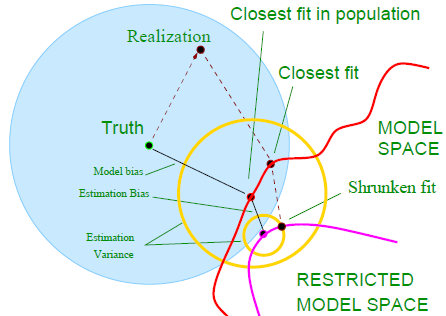
\includegraphics[width=0.5\textwidth]{Figures/BiasVariance}
    \caption{Bias-Variance Relationship}
    \label{fig:}
\end{figure}

\subsection{Optimism of the Training Error Rate}